\documentclass[]{article}
\usepackage{lmodern}
\usepackage{amssymb,amsmath}
\usepackage{ifxetex,ifluatex}
\usepackage{fixltx2e} % provides \textsubscript
\ifnum 0\ifxetex 1\fi\ifluatex 1\fi=0 % if pdftex
  \usepackage[T1]{fontenc}
  \usepackage[utf8]{inputenc}
\else % if luatex or xelatex
  \ifxetex
    \usepackage{mathspec}
    \usepackage{xltxtra,xunicode}
  \else
    \usepackage{fontspec}
  \fi
  \defaultfontfeatures{Mapping=tex-text,Scale=MatchLowercase}
  \newcommand{\euro}{€}
\fi
% use upquote if available, for straight quotes in verbatim environments
\IfFileExists{upquote.sty}{\usepackage{upquote}}{}
% use microtype if available
\IfFileExists{microtype.sty}{%
\usepackage{microtype}
\UseMicrotypeSet[protrusion]{basicmath} % disable protrusion for tt fonts
}{}
\usepackage[a4paper]{geometry}
\usepackage{graphicx}
\makeatletter
\def\maxwidth{\ifdim\Gin@nat@width>\linewidth\linewidth\else\Gin@nat@width\fi}
\def\maxheight{\ifdim\Gin@nat@height>\textheight\textheight\else\Gin@nat@height\fi}
\makeatother
% Scale images if necessary, so that they will not overflow the page
% margins by default, and it is still possible to overwrite the defaults
% using explicit options in \includegraphics[width, height, ...]{}
\setkeys{Gin}{width=\maxwidth,height=\maxheight,keepaspectratio}
\ifxetex
  \usepackage[setpagesize=false, % page size defined by xetex
              unicode=false, % unicode breaks when used with xetex
              xetex]{hyperref}
\else
  \usepackage[unicode=true]{hyperref}
\fi
\hypersetup{breaklinks=true,
            bookmarks=true,
            pdfauthor={Thomas McColgan, Hermann Wagner, Richard Kempter},
            pdftitle={Extracellular potentials generated by axonal projections are shaped by patterns of bifurcations and terminations},
            colorlinks=true,
            citecolor=blue,
            urlcolor=blue,
            linkcolor=magenta,
            pdfborder={0 0 0}}
\urlstyle{same}  % don't use monospace font for urls
\setlength{\parindent}{0pt}
\setlength{\parskip}{6pt plus 2pt minus 1pt}
\setlength{\emergencystretch}{3em}  % prevent overfull lines
\setcounter{secnumdepth}{0}

\title{Extracellular potentials generated by axonal projections are shaped by
patterns of bifurcations and terminations}
\author{Thomas McColgan, Hermann Wagner, Richard Kempter}
\date{\today}

\begin{document}
\maketitle

\section{Introduction}\label{introduction}

Extracellular field potentials (EFPs) are at the heart of many
experimental methods used to examine the inner workings of the brain.
This includes invasive (Local Field Potentials, Current Source Density,
Multiunit Activity) as well as noninvasive (EEG, ECoG, ABR) methods
(Nunez and Srinivasan, 2006; Brette and Destexhe, 2012). The origins of
these EFPs, especially in cases in which the activity is not clearly
attributable to a single cell, is a matter of debate.

EFPs in the brain were long thought to be primarily synaptic in origin
(Buzsáki et al., 2012). As a consequence, many modeling studies focus on
the extracellular fields induced by synaptic currents on the dendrites
and soma of the postsynaptic neuron (Holt and Koch, 1999; Gold et al.,
2006; Lindén et al., 2010, 2011; Einevoll et al., 2013; Fernández-Ruiz
et al., 2013). However, a number of recent data analysis and modeling
efforts have revealed that active, non-synaptic membrane currents can
play an important role in generating EFPs (Ray and Maunsell, 2011;
Belluscio et al., 2012; Schomburg et al., 2012; Reimann et al., 2013;
Anastassiou et al., 2015), including far reaching potentials detectable
at the scalp (Teleńczuk et al., 2011, 2015).

One of the reasons for the traditional assumption that axonal currents
contribute little to the EFP is that the far field of an action
potential traveling along an idealized straight axon is quadrupolar,
meaning that its far field decays faster with distance than synaptic
sources which are thought to be dipolar (Nunez and Srinivasan, 2006).
However, in experimental studies that recorded the EFP of axonal
responses, the EFP often has a dipolar structure. For example, Blot and
Barbour (2014) report an EFP with the characteristic dipolar structure
recorded from the vicinity of cerebellar Purkinje cell axons.

\begin{itemize}
\itemsep1pt\parskip0pt\parsep0pt
\item
  find more examples in literature
\end{itemize}

This discrepancy raises the open question of how axons are able to
generate dipolar field potentials in the actual organism, when
conventional simulation results lead one to expect quardupolar
structures.

The aim of this study is to show how these effects in the EFP of axons
can be explained by the axons' anatomical structure. In particular, we
aim to explain how typical projection patterns in which axons bifurcate
and then terminate in their projection area lead to a dipolar EFP
structure. Such axon bundles, sometimes called nerves or facicles, exist
throughout the peripheral and central nervous system of most animals
(Nornes and Das, 1972; Goodman et al., 1984; Hentschel and Ooyen, 1999;
Kandel et al., 2000). The white matter of the mammalian brain can be
viewed as an agglomeration of such bundles (Schüz and Braitenberg,
2002).

These properties are first investigated by numerical model based on a
forward simulation of the extracellular field potential (Holt and Koch,
1999; Gold et al., 2006). This first model includes a large-scale
multicompartment model of the axon population. We then show a concrete
example of the effects in experimental data using as a set of multi-site
in-vivo electrophysiological recordings from the barn owl brain stem.
Finally, we show the mechanisms underlying the observed effects by means
of a second, analytically tractable, model of a generic axon bundle.
Results ==============

\emph{Axonal projections generate a dipole-like field potential.} To
understand how axons can generate a dipolar EFP, we simulated a parallel
fiber bundle that at first runs at constant diameter and without
bifurcations, then reaches a bifurcation zone with an increasing number
of fibers, and finally reaches a termination zone, in which the number
of fibers decreases to zero. (Figure 1A and 1D). The bundle fibers were
stimulated with a background spontaneous rate, upon which a pulse of
increased activity was added. To characterize the spatiotemporal
dynamics of the evoked EFP, the potential was calculated for several
locations along the axon trunk.

The spatial behaviour of the low-frequency component of the EFP differed
strongly from that of the high-frequency component, so we analyzed them
separately. Low-frequency responses are shown in the top half of Figure
1, and high-frequency responses are shown in the lower half.

The distribution of maximum amplitudes, shown by the contour lines in
Figure 1A, showed the double-lobed shape typical of a dipole, and
exceeds the reach of the high-frequency maximum responses (Fig. 1D). The
low-frequency waveforms (Fig 1B) show a biphasic deflection that is
elicited by the population firing rate pulse. This deflection was
visible at all recoring locations. It reversed polarity in the middle of
the bifurcation zone of the bundle (red box in Figure 1B).

The same distribution of maximum amplitudes for the high-frequency
component, shown in Figure 1D, did not show the same lobed shape.
Instead it decayed much faster with distance in both axial and radial
direction. This was also reflected in the waveforms (Fig 1E). There is
an increase in amplitude due to the firing rate pulse at locations close
to the nerve bundle, but at locations further away from the trunk it is
no longer distinguishable from the background activity.

\begin{figure}[htbp]
\centering
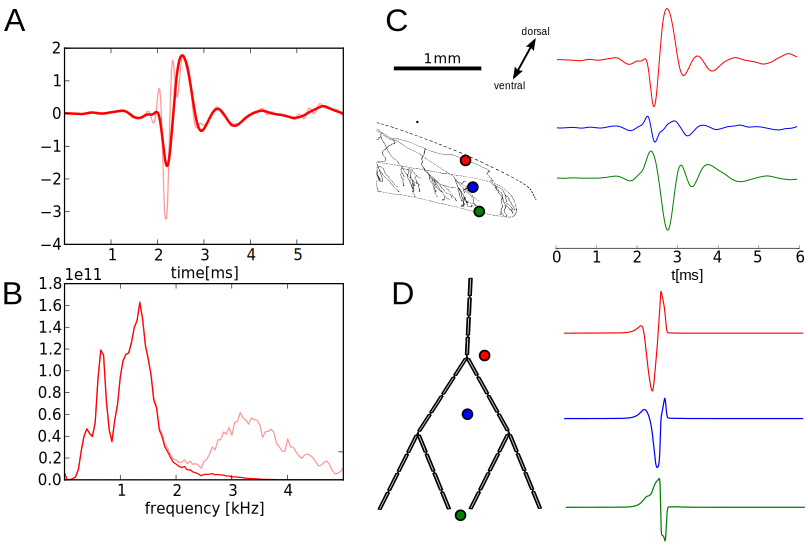
\includegraphics{../figs/fig_1.pdf}
\caption{Axonal projections generate a dipole-like extracellular field
potential (EFP) when stimulated with a pulse of activity. \textbf{A}
shows the modeled axon bundle in black, along with iso-amplitude lines
for the low-pass filtered EFP signature of the activity pulse. The
contours show the typical double-lobe of a dipole. The waveforms,
recorded at the locations of the colored dots in \textbf{A} and shown in
\textbf{B}, also show a polarity reversal. The most salient locations
are highlighted with the red box. The transition ocurrs by inverting the
envelope with aproximately constant phase, not by a shifting of phase
with constant envelope. \textbf{C} shows the progression of the maximum
amplitude with depth (red line). It closely follows the local density of
bifurcations and terminations (black histogram). The situation is
different for the high-frequency component. The iso-amlitude contours
shown in \textbf{D} do not exhibit the same double-lobe structure, and
the waveforms (\textbf{C}) also don't reverse polarity. The amplitude
envelope of the high-frequency component (red line in \textbf{E})
follows the density of fibers (black histogram in \textbf{E}).}
\end{figure}

\emph{Frequency components are related to different anatomical
features.} To better understand the relationship between axonal anatomy
and this spatial structure of the EFP, we plotted the change in density
of the bundle, meaning the number of terminations subtracted from the
number of bifurcations at a given

The low-frequency component shows a distinct relationship to the
anatomy: it appears to be governed by the local density of bifurcations
and terminations. Along the nerve trunk the fiber density is constant,
and the low frequency component is unchanged. As the axon bundle reaches
its projection zone, the number of bifurcations increases, and the low
frequency component increases in amplitude. In the middle of the
projection zone, the number of bifurcations and terminations cancels
out. Correspondingly, the low-frequency component amplitude reaches a
local minimum. As the end of the projection zone approaches, the
terminations outweigh the bifurcations, and the amplitude increases, but
the polarity is reversed (red box in Figure 1B). As the axon bundle
ends, there are no longer any bifurcations or terminations, and the
amplitude decays.

The high-frequency component changes its amplitude in the longitudinal
direction in accordance to the local fiber density. It has an
approximately constant amplitude along the nerve trunk and then
increases in amplitude as the fiber density is increased by
bifurcations. As the fibers terminate and fiber density decreases, so
does the amplitude of the high-frequency component.

These relationships suggest that the particular structure of the axon
bundle gives rise to the dipolar field potential. Because dipolar fields
are associated with a longer spatial reach that the quarupolar fields
typically associated with axonal spikes, we decided to investigate the
effect that axon structure has on the spatial reach of the frequency
components. To do this we performed a further simulation of an axon
bundle, this time omitting the bifurcations, and letting the fibers
terminate directly. The resulting distance decay profiles are shown in
Figure 2. In axial direction, the low-frequency component has a further
reach than the high frequency component in the bifurcating case (Figure
2A), but not in the non-bifurcating case (Figure 2C). In the radial
direction, the situation is different: the bifurcating (Figure 2B) and
non-bifurcating (Figure 2D) case both show a faster decay of the
high-frequency component than of the low-frequency component. To assure
that the effect was due to the bifurcations themselves and not due to
the fanned out structure of the bifurcating bundle seen in Figures 2A
and 2D, we here changed the layout of both bundles to have constant
widths.

\begin{figure}[htbp]
\centering
\includegraphics{../figs/fig_2.pdf}
\caption{Low-frequency component of the axon bundle EFP exceeds
high-frequency component in reach, modulated by axon structure. All
plots show the scaling of the low-frequency (blue lines) and
high-frequency (green lines) frequency components on a
doubly-logarithmic scale. Amplitudes were normalized to unit value at
the end of the tuft in axial direction (\textbf{A} and \textbf{C}) and
from the trunk in radial direction (\textbf{B} and \textbf{D}).
\textbf{A} and \textbf{B} show the behaviour in the case of a
bifurcating bundle, while \textbf{C} and \textbf{D} show the
nonbifurcating case. In the bifurcating case, the low-frequency
component exceeds the reach of the high-frequency comonent in both
directions. In the non-bifurcating case, the decay is the same for both
components in the axial direction. This is consistent with the presence
of a low-frequency dipole-like potential in the bifurcating bundle but
not in the non-bifurcating bundle.}
\end{figure}

\emph{The barn owl neurophonic as an example that shows these
properties.} In order to test our model of the extracellular field of
axon bundles, we compared it to recordings from the barn owl auditory
brain stem. We adjusted the model parameters to match the anatomy and
physiology of nucleus laminaris (NL), and set the activation statistics
to match measured PSTHs in response to stimulation by a click sound
presented to one ear. We then simulated the resulting EFP at varying
depths, corresponding to recording depths in the experiment. The
resulting recordings from experiment and simulation are shown in Figure
3.

The simulated EFPs showed several characteristics that are also observed
in the data. Firstly, the high-frequency component shows a steady
increase in latency along the projections' depth, and has its maximum in
amplitude in the middle of NL. The low-frequency component reverses
polarity along the depth of NL, and almost vanishes in the middle of NL.
This is the same behaviour as shown for the generic axon bundle in the
previous section.

It is interesting to note that a similar reversal of polarity in NL has
been reported for chicken (Schwarz, 1992), as well as in the mamalian
analog to NL, the medial superior olive (Laughlin et al., 2010). The
phase reversal in this case has been modeled based on the assumption
that the postsynaptic NL and MSO dendrites with their bipolar morphology
have a dipolar EFP response (Laughlin et al., 2010; Goldwyn et al.,
2014). However, in the owl this dipolar morphology is largely absent
(Carr and Konishi, 1990), making dendritic sources unlikely.

\begin{figure}[htbp]
\centering
\includegraphics{../figs/fig_3.pdf}
\caption{Data from the barn owl shows the expected behaviour predicted
by the model. (\textbf{A},\textbf{B}) shows data from the barn owls
nucleus laminaris in response to an auditory click stimulus, compared to
a simulation of the axonal structure and activation in
(\textbf{C},\textbf{D}). The click stimulus induces a pulse of activity
in the afferent axon bundle. The low-frequency components (\textbf{A}
and \textbf{C}) show the polarity reversal. The high frequency component
(\textbf{B} and \textbf{D}), does not show such a reversal, but rather
shows a steady increase in phase with depth.}
\end{figure}

\emph{Mechanism underlying the observed properties I.} We begin by
looking at the response of a single axon tree to a single spike at
various locations along the tree, as shown in Figure 4. This can already
give us a rough idea about the origin of the observed polarity reversal.

The extracellular response at a recording location along a continuation
of the axon, i.e.~not close to a bifurcation or termination, is
triphasic (blue trace in Figure 4B). It has been noted that this shape
is approximated by the second derivative of the membrane voltage: the
first positive peak is the initial bend to the rising flank of the
action potential, the main dip corresponds to the high curvature at the
peak of the action potential, and the final, positive peak corresponds
to the bend from hyperpolarization to recovery.

The potential near a bifurcation (red trace in Figure 4B) has a more
biphasic shape. There is a small initial peak, but the response is
dominated by the second, negative and the third, positive peak. This can
be understood by comparing the shape to the previous example along a
non-bifurcating axon: The initial shape resembles the non-bifurcating
case, because the action potential is still mainly within the segments
before the bifurcation. As the action potential passes the bifurcation,
there are now two instances of the action potential, and the second and
third peak are doubled in size, leading to the more biphasic response.

The same reasoning can be applied to the case of the biphasic response
at a termination (green trace in Figure 4B): here there is an
approaching action potential, leading to an initial positive peak, but
as the termination is reached, the current flow ceases, and there is
only a reduced second peak, and the third peak, associated with the
action potential moving away from the recording location, disappears
completely.

A notable point here is that the potential at the bifurcation and
termination are similar in shape, but opposite in polarity. This
resembles the observed polarity reversal. It is thus not hard to imagine
that this effect is caused by the response being dominated by
bifurcations in the early part of NL where the axons branch out, and
then by terminations in the later part, where terminations are more
prevalent, with the two canceling out in the middle. We will test this
intuition in the following by examining the properties of a full bundle
of axons in a simplified analytical model.

\begin{figure}[htbp]
\centering
\includegraphics{../figs/mockups/fig4.pdf}
\caption{The dipolar behaviour can be understood by examining individual
action potentials on a single axon tree. Comparing the low frequency owl
data (\textbf{A}) to a single axon and action potential in model
(\textbf{B}) shows a similar behaviour. In particular, the potential at
a termination and that at a bifurcation (red and green curves in
\textbf{B}) are approximately inverted.}
\end{figure}

\emph{Mechanism underlying the observed properties II.} In the case of a
simplified one-dimensional axon bundle, the EFP at a given location may
be described by the formula
\(\Phi(\mathbf{r},t) = \left[\left\{n(z)\cdot i_\lambda(z,t)\right\}\ast w(a,z)\right]_z\)
(see Methods and appendix). Assuming that the weighting function \(w\)
tends to 0 for large \(\left|z\right|\), and with the introduction of
the single axon current integral
\(I_\lambda(z,t)=\int_{-\infty}^zi_\infty(z',t)dz'\), the equation can
be split (for a derivation, see appendix) into two components:

\begin{align}
  \label{eqn:splitpot} 
  \Phi(\mathbf{r},t) = &\left[\left\{n(z)\cdot I_\lambda(z,t)\right\}\ast w'(\rho,z)\right]_z \\
  & - \left[\left\{n'(z)\cdot I_\lambda(z,t)\right\}\ast w(\rho,z)\right]_z 
\end{align}

In the first component the single axon current integral
\(I_\lambda(z,t)\) is multiplied by the local density of the fibers
\(n\), while the weighting function is replaced by its spatial
derivative \(w'\). In the second component, \(I_\lambda\) is multiplied
by the derivative of the density \(n'\), but here the weighting function
\(w\) is unchanged. The functions \(w\) and \(w'\) are shown in the time
and frequency domain in Figure 4.

Further inspection of the two components shows an intriguing similarity
to the properties of the response observed in the previous sections. The
first component is high-pass filtered, and is related to the fiber
density, just like `noise' component in Figure 1 and the high-frequency
component in the barn owl data and model. The second component is
low-pass filtered, and related to the derivative of the fiber density,
just like the firing rate pulse related deflection in Figure 1, and the
low-frequency component in the barn owl.

\begin{itemize}
\itemsep1pt\parskip0pt\parsep0pt
\item
  Add simplified explanations of:
\item
  spatial filtering
\item
  dipole/stationary potentials
\end{itemize}

\begin{figure}[htbp]
\centering
\includegraphics{../figs/mockups/fig5.pdf}
\caption{Analytical model of the axon bundle potential explains the
effects observed in the numerical model and example data. (\textbf{A})
shows the behaviour of a simplified fiber bundle with a piecewise
constant fiber density (\textbf{Aa}). The high-frequency component
(\textbf{Ab}) shows no polarity reversal, while the low-frequency
component (\textbf{Ac}) does, as expected from the data and modeling.
This can be understood by decomposing the signal into two components.
The first component is governed by the bifurcation and termination
density, and is filtered by the regular weighting function
(\textbf{Ba}), which acts as a low-pass filter (\textbf{Bb}). The second
component is governed by the fiber density, and is filtered by the
derivative of the weighting function (\textbf{Bc}), which acts as a
high- or band-pass filter (\textbf{Bd}).}
\end{figure}

\section{Discussion}\label{discussion}

\begin{itemize}
\itemsep1pt\parskip0pt\parsep0pt
\item
  Relevance of Findings

  \begin{itemize}
  \itemsep1pt\parskip0pt\parsep0pt
  \item
    Interpretation of CSD

    \begin{itemize}
    \itemsep1pt\parskip0pt\parsep0pt
    \item
      Classical CSD: constant fiber density, variable currents
    \item
      Here: variable fiber density, constant currents
    \end{itemize}
  \item
    Dipole has far field, ABR response?
  \end{itemize}
\item
  Compare to other auditory systems (Chicken NL, MSO)

  \begin{itemize}
  \itemsep1pt\parskip0pt\parsep0pt
  \item
    Speculate on functional relevance of polarity shift (a la Rinzel \&
    Goldwyn, Weiss 2010, Einevoll\&Panzeri review)
  \end{itemize}
\item
  Two simultaneous modes: stationary dipole and continuous (cf Mc
  Laughlin, etc).
\item
  compare to other fiber bundle systems
\end{itemize}

\section{Methods}\label{methods}

\subsection{Experimental recordings}\label{experimental-recordings}

\subsection{Numerical model}\label{numerical-model}

We modeled the axons using NEURON (Hines and Carnevale, 1997; Hines et
al., 2009) in a model based on previous work by (\textbf{refs}),
including the high and low threshold potassium channels used by
(\textbf{refs}). The axon was modeled as a sequence of active nodes and
passive myelinated segments. The parameters for the active and passive
segments are described in Table \ref{tab:modparam}. Unlike previous
models, we included branching axons in our simulations. These were
generated by connecting two passive segments to a node, and continuing
the alternation of active and passive segment in each resulting branch.

Action potentials were initiated in the axons by injecting a current
pulse into the first node of Ranvier of the axon. The times of the
injections were chosen by drawing from an inhomogeneous Poisson
distribution based on the firing statistics of NM units in response to a
given stimulus.

\begin{itemize}
\itemsep1pt\parskip0pt\parsep0pt
\item
  Split barn owl and general axon bundle
\end{itemize}

Axon branching patterns were generated procedurally, \textbf{better
wording} starting with the root segment, placed at the border of NL. In
order to avoid artifacts from the current pulse injection and to
simulate the fiber tract leading up to NL, a sequence of 10 active and
passive segments without bifurcations was added before the root. To this
root, segments were appended iteratively. Before adding a segment, a
decision whether to branch or terminate an axon was drawn from a
probability distribution dependent on the dorsoventral depth of the end
of the previous segment. These probability distributions were modeled as
logistic functions with the parameters adjusted to roughly match the
numbers of branchings and terminations found in the tracings shown in
publications such as Carr and Konishi (1990). This meant that an initial
phase of bifurcations was followed by a phase of terminations, with the
probability of termination reaching 100\% at the end of NL.

The simulations of these axons yielded the membrane currents, from which
we calculated the extracellular fields. The procedure for this is
described in detail by Gold et al. (2006), among others. Briefly, the
extracellular medium is assumed to be a homogeneous volume conductor
with conductivity \(\sigma_e\), and a quasi-static approximation of the
electrical field potential \(\phi\) is made. The extracellular potential
due to a current distribution \(i(\mathbf{r},t)\) is then governed by
the equation \(\Delta \phi = \frac{1}{\sigma_e} i(\mathbf{r},t)\), with
\(\Delta\) denoting the Laplace operator. If the currents \(i\) are
constrained to a volume \(V\), this equation has the solution:

\begin{equation}
  \phi(\mathbf{r},t)=\frac{1}{4\pi\sigma_{e}}\int_{V}\frac{i(\mathbf{r}',t)}{|\mathbf{r}-\mathbf{r}'|}\textrm{d}\mathbf{r}'
  \label{eqn:basic}
\end{equation}

Since the currents though the myelinated segments were negligible, and
the nodes of Ranvier are small, we used the point source approximation
of only the node currents, and did not include the line source
approximation used by Holt and Koch (1999).

\begin{table}[h]
  \begin{centering}
    \begin{tabular}{|c|c|}
      \hline 
      parameter & value\tabularnewline
      \hline 
      \hline 
      $g_{\text{Na}}$ & 0.8 S/cm\texttwosuperior{}\tabularnewline
      \hline 
      $g_{\text{KLVA}}$ & 0.1 S/cm\texttwosuperior{}\tabularnewline
      \hline 
      $g_{\text{KHVA}}$ & 1.5 S/cm\texttwosuperior{}\tabularnewline
      \hline 
      $C_{\text{mem}}$ & 1.0 $\mu$F/cm\texttwosuperior{}\tabularnewline
      \hline 
    \end{tabular}
    \par
  \end{centering}
  \caption{Model Parameters **add: leak conductance, myelin parameters, extracellular conductivity sizes**}
  \label{tab:modparam}
\end{table}

\subsection{Simplified axon bundle
model}\label{simplified-axon-bundle-model}

\label{sec:efpresp}

We define the spatial dimension in cylindrical coordinates
\(\mathbf{r}=(\rho,\varphi,z)\) such that \(z\) is the dorsoventral
direction, increasing from dorsal to ventral, and \(z=0\) is the dorsal
border of NL. We further define \(\hat{\mathbf{e}}_{z}\) as the unit
vector in \(z\) direction, and \(\hat{\mathbf{e}}_{\rho}\) as an
arbitrary unit vector perpendicular to the \(z\) direction.

Let us first consider a simple model axon that extends infinitely on
both sides and in a straight line from the dorsal direction into NL, and
at 0 in the remaining coordinates. Furthermore, we consider a single
action potential propagating along this axon. This axon then has a
non-zero current density only at \(\rho=0\), which we denote
\(i_{\infty}(z,t)\), meaning that in this case
\(i(\mathbf{r},t)=\delta(\rho)i_{\infty}(z,t)\). Applying this to
equation \ref{eqn:basic}, corresponding response
\(\kappa_{\infty}(\mathbf{r},t)\) of an action potential propagating
through such a line-axon is then

\begin{align}
\kappa_{\infty}(\mathbf{r},t) & =\frac{1}{4\pi\sigma_{e}}\int_{V}\frac{\delta(\rho')i_{\infty}(z',t)}{|\mathbf{r}-\mathbf{r}'|}\textrm{d}\mathbf{r}'\label{eq:halfline}\\
& =\frac{1}{4\pi\sigma_{e}}\int_{-\infty}^{\infty}\frac{i_{\infty}(z',t)}{|\mathbf{r}-z'\hat{\mathbf{e}}_{z}|}\textrm{d}z'
\end{align}

We will call this response a spike kernel because it will take the role
of an integral kernel in the following.

Due to the rotational symmetry, the kernel at a distance \(\rho\) from
the axon, regardless of \(\varphi\), can then be described by

\begin{align} \label{eqn:infkern}
\kappa_{\infty}(\mathbf{r},t) & =\frac{1}{4\pi\sigma_{e}}\int_{-\infty}^{\infty}\frac{i_{\infty}(z',t)}{|(z-z')\hat{\mathbf{e}}_{z} + \rho\hat{\mathbf{e}}_{\rho}|}\textrm{d}z' \\
& =\frac{1}{4\pi\sigma_{e}}\int_{-\infty}^{\infty}\frac{i_{\infty}(z',t)}{\sqrt{(z-z')^2 + \rho^2}}\textrm{d}z' 
\end{align}

Equation \ref{eqn:infkern} has the form of a convolution with a
weighting function \(w\):

\begin{equation}
  w(\rho,z) = \frac{1}{4\pi\sigma_e}\frac{1}{\sqrt{z^2+\rho^2}}
  \label{eqn:weighting}
\end{equation}

The convolution can then be written as:

\begin{equation}
\kappa_{\infty}(\mathbf{r},t) = \left[i_{\infty}(z,t)\ast w(\rho,z)\right]_z
\end{equation}

with the operator \(\left[\cdot\ast\cdot\right]_z\) denoting the
convolution with respect to the variable \(z\).

The simplest model of a terminating axon will be a semi-infinite axon,
where the membrane current flow is simply set to zero beyond the
termination point \(z_\text{term}\). Using the Heaviside step function
\(H\) we find kernel \(\kappa_{\text{term}}\) of a spike in a
terminating axon:

\begin{equation}
  \kappa_{\text{term}}(\mathbf{r},t) = \left[\left\{H(z_\text{term}-z)\cdot i_{\infty}(z,t)\right\}\ast w(\rho,z)\right]_z
\end{equation}

Similarly, the model of a bifurcating axon would be one in which the
current flow after the bifurcation point \(z_\text{bif}\) is double that
of the single infinite fiber.

\begin{equation}
  \kappa_{\text{bif}}(\mathbf{r},t) = \left[\left\{\left(1+H(z-z_\text{bif})\right)\cdot i_{\infty}(z,t)\right\}\ast w(\rho,z)\right]_z
\end{equation}

This places the child branches in superposition at \(\rho=0\), which is
a useful approximation for small branching angles.

Approximating terminations and bifurcations in this way disregards the
boundary effects that may appear due to the conservation of charge and
the inability of charge to flow beyond the termination. However, since
the integral over \(i_\infty\) is zero for realistic action potentials,
the conservation of charge is maintained in the long run.

In more general terms, a coherently stimulated axon bundle with
terminations and bifurcations along it's path can be described by the
number of individual fibers \(n(z)\) at any depth. The extracellular
potential \(\kappa_\text{b}\) of such a bundle in which the action
potential is initiated at the same time and location is then given by

\begin{equation}
  \kappa_{\text{b}}(\mathbf{r},t) = \left[\left\{n(z)\cdot i_{\infty}(z,t)\right\}\ast w(\rho,z)\right]_z
  \label{eqn:bundlekern}
\end{equation}

If we want to calculate the combined field of many axons and action
potentials, we can do so by linearly summing the individual axon fields.

If all axons in the bundle are driven with the same the mean firing rate
\(\lambda(t)\), which might be modulated in time, the field potential
\(\Phi(\mathbf{r},t)\) in response to this firing rate will be the
(temporal) convolution of the firing rate with the response of the
bundle to a coherent spike in all axons:

\begin{equation}
  \Phi(\mathbf{r},t) = \left[\kappa_\text{b}(\mathbf{r},t) \ast \lambda(t)\right]_t
  \label{eqn:fullpot}
\end{equation}

Substituting equation \ref{eqn:bundlekern} into equation
\ref{eqn:fullpot}, and taking advantage of the fact that only
\(i_\infty\) and \(\lambda\) depend on \(t\) gives

\begin{align}
  \label{eqn:switchedpot}
  \Phi(\mathbf{r},t) & =  \left[\left[\left\{n(z)\cdot i_{\infty}(z,t)\right\}\ast w(\rho,z)\right]_z \ast \lambda(t)\right]_t \\
  & =  \left[\left\{n(z)\cdot \left[i_{\infty}(z,t)\ast \lambda(t)\right]_t\right\}\ast w(\rho,z)\right]_z
\end{align}

With the average current in a single infinite fiber stimulated with
\(\lambda\), which we will denote it with
\(i_\lambda(z,t) := \left[i_{\infty}(z,t)\ast \lambda(t)\right]_t\) this
gives us

\begin{align}
  \Phi(\mathbf{r},t) & =  \left[\left\{n(z)\cdot i_\lambda(z,t)\right\}\ast w(a,z)\right]_z
  \label{eqn:switchedpotend}
\end{align}

\section*{Bibliophraphy}\label{bibliophraphy}
\addcontentsline{toc}{section}{Bibliophraphy}

\hyperdef{}{ref-Anastassiou2015Cell}{}
Anastassiou CA, Perin R, Buzsáki G, Markram H, Koch C (2015) Cell type-
and activity-dependent extracellular correlates of intracellular
spiking. Journal of Neurophysiology 114:608--623 Available at:
\url{http://dx.doi.org/10.1152/jn.00628.2014}.

\hyperdef{}{ref-Belluscio2012CrossFrequency}{}
Belluscio MA, Mizuseki K, Schmidt R, Kempter R, Buzsáki G (2012)
Cross-Frequency Phase--Phase Coupling between Theta and Gamma
Oscillations in the Hippocampus. The Journal of Neuroscience 32:423--435
Available at: \url{http://dx.doi.org/10.1523/jneurosci.4122-11.2012}.

\hyperdef{}{ref-Blot2014Ultrarapid}{}
Blot A, Barbour B (2014) Ultra-rapid axon-axon ephaptic inhibition of
cerebellar Purkinje cells by the pinceau. Nat Neurosci 17:289--295
Available at: \url{http://dx.doi.org/10.1038/nn.3624}.

\hyperdef{}{ref-Brette2012Handbook}{}
Brette R, Destexhe A eds. (2012) Handbook of Neural Activity
Measurement. Cambridge: Cambridge University Press. Available at:
\url{http://dx.doi.org/10.1017/cbo9780511979958}.

\hyperdef{}{ref-Buzsaki2012Origin}{}
Buzsáki G, Anastassiou CA, Koch C (2012) The origin of extracellular
fields and currents--EEG, ECoG, LFP and spikes. Nature reviews
Neuroscience 13:407--420 Available at:
\url{http://dx.doi.org/10.1038/nrn3241}.

\hyperdef{}{ref-carr90}{}
Carr CE, Konishi M (1990) A circuit for detection of interaural time
differences in the brain stem of the barn owl. The Journal of
Neuroscience 10:3227--3246 Available at:
\url{http://www.jneurosci.org/content/10/10/3227.abstract}.

\hyperdef{}{ref-Einevoll2013Modelling}{}
Einevoll GT, Kayser C, Logothetis NK, Panzeri S (2013) Modelling and
analysis of local field potentials for studying the function of cortical
circuits. Nature reviews Neuroscience 14:770--785 Available at:
\url{http://dx.doi.org/10.1038/nrn3599}.

\hyperdef{}{ref-FernandezRuiz2013Cytoarchitectonic}{}
Fernández-Ruiz A, Muñoz S, Sancho M, Makarova J, Makarov VA, Herreras O
(2013) Cytoarchitectonic and Dynamic Origins of Giant Positive Local
Field Potentials in the Dentate Gyrus. The Journal of Neuroscience
33:15518--15532 Available at:
\url{http://dx.doi.org/10.1523/jneurosci.0338-13.2013}.

\hyperdef{}{ref-Gold2006Origin}{}
Gold C, Henze DA, Koch C, Buzsáki G (2006) On the origin of the
extracellular action potential waveform: A modeling study. Journal of
neurophysiology 95:3113--3128 Available at:
\url{http://dx.doi.org/10.1152/jn.00979.2005}.

\hyperdef{}{ref-Goldwyn2014Model}{}
Goldwyn JH, Laughlin MM, Verschooten E, Joris PX, Rinzel J (2014) A
Model of the Medial Superior Olive Explains Spatiotemporal Features of
Local Field Potentials. The Journal of Neuroscience 34:11705--11722
Available at: \url{http://dx.doi.org/10.1523/jneurosci.0175-14.2014}.

\hyperdef{}{ref-Goodman1984Cell}{}
Goodman CS, Bastiani MJ, Doe CQ, Lac S du, Helfand SL, Kuwada JY, Thomas
JB (1984) Cell recognition during neuronal development. Science (New
York, NY) 225:1271--1279 Available at:
\url{http://view.ncbi.nlm.nih.gov/pubmed/6474176}.

\hyperdef{}{ref-Hentschel1999Models}{}
Hentschel HGE, Ooyen A van (1999) Models of axon guidance and bundling
during development. Proceedings of the Royal Society of London B:
Biological Sciences 266:2231--2238 Available at:
\url{http://dx.doi.org/10.1098/rspb.1999.0913}.

\hyperdef{}{ref-Hines1997NEURON}{}
Hines ML, Carnevale NT (1997) The NEURON Simulation Environment. Neural
Computation 9:1179--1209 Available at:
\url{http://dx.doi.org/10.1162/neco.1997.9.6.1179}.

\hyperdef{}{ref-Hines2009NEURON}{}
Hines ML, Davison AP, Muller E (2009) NEURON and Python. Frontiers in
neuroinformatics 3 Available at:
\url{http://dx.doi.org/10.3389/neuro.11.001.2009}.

\hyperdef{}{ref-Holt1999Electrical}{}
Holt GR, Koch C (1999) Electrical Interactions via the Extracellular
Potential Near Cell Bodies. Journal of Computational Neuroscience
6:169--184 Available at:
\url{http://dx.doi.org/10.1023/a:1008832702585}.

\hyperdef{}{ref-kandel2000principles}{}
Kandel ER, Schwartz JH, Jessell TM, Others (2000) Principles of neural
science. McGraw-Hill New York.

\hyperdef{}{ref-Laughlin2010Oscillatory}{}
Laughlin MM, Verschooten E, Joris PX (2010) Oscillatory Dipoles As a
Source of Phase Shifts in Field Potentials in the Mammalian Auditory
Brainstem. The Journal of Neuroscience 30:13472--13487 Available at:
\url{http://dx.doi.org/10.1523/jneurosci.0294-10.2010}.

\hyperdef{}{ref-Linden2010Intrinsic}{}
Lindén H, Pettersen K, Einevoll G (2010) Intrinsic dendritic filtering
gives low-pass power spectra of local field potentials. Journal of
computational neuroscience 29:423--444 Available at:
\url{http://dx.doi.org/10.1007/s10827-010-0245-4}.

\hyperdef{}{ref-Linden2011Modeling}{}
Lindén H, Tetzlaff T, Potjans TC, Pettersen KH, Grün S, Diesmann M,
Einevoll GT (2011) Modeling the Spatial Reach of the LFP. Neuron
72:859--872 Available at:
\url{http://dx.doi.org/10.1016/j.neuron.2011.11.006}.

\hyperdef{}{ref-Nornes1972Temporal}{}
Nornes HO, Das GD (1972) Temporal pattern of neurogenesis in spinal
cord: cytoarchitecture and directed growth of axons. Proceedings of the
National Academy of Sciences of the United States of America
69:1962--1966 Available at:
\url{http://view.ncbi.nlm.nih.gov/pubmed/4114859}.

\hyperdef{}{ref-Nunez2006Electric}{}
Nunez PL, Srinivasan R (2006) Electric Fields of the Brain. Oxford
University Press. Available at:
\url{http://dx.doi.org/10.1093/acprof:oso/9780195050387.001.0001}.

\hyperdef{}{ref-Ray2011Different}{}
Ray S, Maunsell JHR (2011) Different Origins of Gamma Rhythm and
High-Gamma Activity in Macaque Visual Cortex. PLoS Biol 9:e1000610+
Available at: \url{http://dx.doi.org/10.1371/journal.pbio.1000610}.

\hyperdef{}{ref-Reimann2013Biophysically}{}
Reimann MW, Anastassiou CA, Perin R, Hill SL, Markram H, Koch C (2013) A
Biophysically Detailed Model of Neocortical Local Field Potentials
Predicts the Critical Role of Active Membrane Currents. Neuron
79:375--390 Available at:
\url{http://dx.doi.org/10.1016/j.neuron.2013.05.023}.

\hyperdef{}{ref-Schomburg2012Spiking}{}
Schomburg EW, Anastassiou CA, Buzsáki G, Koch C (2012) The Spiking
Component of Oscillatory Extracellular Potentials in the Rat
Hippocampus. The Journal of Neuroscience 32:11798--11811 Available at:
\url{http://dx.doi.org/10.1523/jneurosci.0656-12.2012}.

\hyperdef{}{ref-Schuz2002Human}{}
Schüz A, Braitenberg V (2002) The Human Cortical White Matter. In:
Cortical areas (Schüz A, ed), pp 377--386. Abingdon, UK: Taylor \&
Francis. Available at:
\url{http://dx.doi.org/10.4324/9780203219911/_chapter/_16}.

\hyperdef{}{ref-Schwarz1992Can}{}
Schwarz DW (1992) Can central neurons reproduce sound waveforms? An
analysis of the neurophonic potential in the laminar nucleus of the
chicken. The Journal of otolaryngology 21:30--38 Available at:
\url{http://view.ncbi.nlm.nih.gov/pubmed/1564747}.

\hyperdef{}{ref-Telenczuk2011Highfrequency}{}
Teleńczuk B, Baker SN, Herz AVM, Curio G (2011) High-frequency EEG
covaries with spike burst patterns detected in cortical neurons. Journal
of Neurophysiology 105:2951--2959 Available at:
\url{http://dx.doi.org/10.1152/jn.00327.2010}.

\hyperdef{}{ref-Telenczuk2015Correlates}{}
Teleńczuk B, Baker SN, Kempter R, Curio G (2015) Correlates of a single
cortical action potential in the epidural EEG. NeuroImage 109:357--367
Available at: \url{http://dx.doi.org/10.1016/j.neuroimage.2014.12.057}.

\end{document}
